\section{Naive Implementation of the Verification Method}
\label{naive}
In this chapter, we show how the algorithm in \ref{verificationalgorithm} could be implemented. The implementation is naïve, it strictly follows the mathematical concepts. Then we identify the main drawbacks of this naïve implementation and suggest some improvements.

\subsection{Definitions and Notations}
In this chapter, we introduce the term \e{potential concretizations}. The reason for the introduction of this term recides in the fact that there is no easy way to directly compute the set of concretizations corresponding to a set of views, i.e. from a set $X_k$ of configurations of size at most $k$ finding $\gamma(X_k)$ of concretizations of size at most $k+1$. Instead, in order to find the concretizations, we generate all of the \e{potential} concretizations, such that a potential configuration is any configuration $con$, $size(v) < size(con) \leq k+1$ for some $v \in X_k$, i.e. any extension of a view already in the set with any symbol in the alphabet.

We maintain a set $X_k$ of views, and denote its state in a specific iteration of algorithm \ref{verificationalgorithm} by $X_k^i$ , such that $X_k^0$ = $\{c^0\}$ and $X_k^m$ = $V_k$ for some $m$.
 
A view $v\in X_k$ may be extended with a symbol on one or more of its channels, yielding the potential concretization $con$. We say that $con$ is \e{accepted}, if all the views of $con$ of size up top $k$ are in $X_k$, otherwise, $con$ is \e{refuted}. 

As an example, let $\conf{s, a, b} \in X_k^i$, then $\conf{s, a, bb}$ is a potential configuration. We say that $con$ is \e{accepted}, if $\alpha_k(con) \subseteq X_k^i$, otherwise, $con$ is \e{refuted}. Note that if $\alpha_k(con) \not\subseteq X_k^i$, there may be $X_k^j$, $i < j$ such that $\alpha_k(con) \subseteq X_k^j$, i.e. a potential configuration may be refuted in one iteration, but accepted in another.

We say that the an accepted concretization $con$ is \e{reached} from the view $v$.

\subsection{Naïve implementation}
\label{apost}
A naïve way of implementing algorithm \ref{verificationalgorithm} would be to implement it in a way that corresponds exactly to the mathematical notations. This is possible to do, as most programming languages have built-in data structures that support set operations. We maintain a \e{set} $X_k = \{v | size(v) \leq k\}$ of views such that all views are uniquely stored in $X_k$, and we will assume that an alphabet $\Sigma$, the set $Bad$ of bad states and a set of transitions $\delta$ are known. The the implementation of the algorithm performs three tasks:

\begin{enumerate}
\item
Compute the set $\mathcal{R}_k$ of reachable configurations of size up to k, used on line 2 of algorithm \ref{verificationalgorithm}. In section \ref{part2} we show how to compute the set $\mathcal{R}_k$.

\item
Compute the set $V_k$ of configurations, i.e. the fixpoint of $X_k$. We know that such a fixpoint exists, due to the Knaster-Tarski theorem\cite{tarski}, and we compute it by iteratively applying the Abstract post-image of $X_k$. This is used on line 3 of algorithm \ref{verificationalgorithm}. The procedure is explained in section \ref{part1}.
\todo[inline]{You commented a while ago that I should reference the Kleene iteration here. I'm really not traversed at all on order theory, but is the difference between the Kleen iteration and the Knaster-Tarski theorem that large, that it merits them both to be mentioned? I fail to see why the result of the Knaster-Tarski theorem would not suffice.}
%\todo[inline]{Note to self: Mention the Kleen iteration in section 2.1.2 and reference it here}
%Now to compute it, we need only to compute the concretisation of size size at most k+1 and then the fixpoint can be compute  using the Kleen iteration...
\item
We need to be able to compute the intersection of a set of configurations with the set $Bad$ of bad configurations. This is done on line 2 and 4 of algorithm \ref{verificationalgorithm}. The procedure is explained below in section \ref{part3}.
\end{enumerate}

\subsubsection{Abstract Post-image}
\label{part1}
In order to compute the abstract post-image $\gamma_k^{k+1}$ of a set $X_k^i$, the concretization function, the post-image and the abstraction functions below are applied in order on $X_k^i$:


\begin{enumerate}
\item
\textbf{Concretization function}:
Generate the set $\gamma_k^{k+1}(X_k^i)$. For each view \e{v} $\in$ $X_k^i$, generate all potential concretizations \e{con}. Then $con \in \gamma_k^{k+1}(X_k)$ if $\alpha_k(con) \subseteq X_k^i$.

%For any such potential concretization \e{con} of size at most $k+1$, remove those for which $\alpha_k(con)$ $\not\subseteq$ $X_k$.
This results in the set of accepted potential concretizations.

\item
\textbf{Post-image}:
\todo[inline]{I added a definition of r(c) in section 2.3}
Generate the set $\rho(\gamma_k^{k+1}(X_k^i))$: For every concretization $con$ $\in$ $\gamma_k^{k+1}(X_k^i)$, $r$ $\in$ $\delta$, $r(con) \in post(\gamma_k^{k+1}(X_k^i))$, i.e. the post-image of the concretization $con$.

\item
\textbf{Abstraction Function}:
Generate $Apost(X_k^i)$: For each \e{c} $\in$ $\rho(\gamma_k^{k+1}(X_k^i))$, compute $\alpha_k(c)$. Let $V' = \{\alpha_k(c)|c \in \rho(\gamma_k^{k+1}(X_k^i))\}$ of views of size at most \e{k}. Then $X_k^{i+1} = X_k^i \cup V'$. If $X_k^i$ = $X_k^{i+1}$, a fixpoint has been reached.

\todo[inline]{You said I should comment that calculating $alpha_k(c)$ is easy. It's technically easy, but not computationally (but it becomes easy later, when I redefine the subword relation)}
%Computing $\alpha_k(c)$ for a concretization $c$ is easy, as finding views $v \subword c$ is easy. 
\end{enumerate}

\subsubsection{Reachable configurations, $\mathcal{R}_k$}
\label{part2}
On line 2 of algorithm \ref{verificationalgorithm}, the set of all reachable configurations of size up to $k$, $\mathcal{R}_k$, is required. Computing the set $\mathcal{R}_k$ can be done in a multitude of ways. A simple way is to iteratively calculate the post-image of each configuration in the set, while taking the buffer size into account.

Let $\rho_k(X)$ be defined such that if given the set of transitions $\delta$, for a configuration $c \in X$ and each transition $r \in \delta$, $r(c) \in \rho_k(X)$ if $size(r(c)) \leq k$. Otherwise, if $size(r(c)) = l > k$, there is a buffer overflow. We assume that such an overflow is handled by removing the last $l-k$ symbols of the word, i.e., if $c = \conf{s, w_1, w_2,..., w_i, ...,  w_m}$ with $w_i = a_1a_2...a_ka_{k+1}...a_l$ is reached, the configuration $c' = \conf{s, w_1, w_2, ..., w_i', ..., w_n}$ with $w_i' = a_1a_2...a_k$ is a member of $\rho_k(X)$.

Let $R_0$ denote the set containing the initial configuration $\conf{s^0, \xi^0}$, and let $R_i = R_{i-1} \cup \rho_k(R_{i-1})$. Then $R_m = \mathcal{R}_k$ for some $m$.

\subsubsection{Checking for bad configurations}
\label{part3}
A bad configuration is any configuration which is in a \e{state} considered to be bad, independent of the channel evaluation. Thus, the set $Bad$ can be expressed as a minimal state of configurations, such that a bad configuration $b \in Bad$ is of the format $b = (s, \xi^0)$. Checking for bad configurations can be done for each configuration $c = (s, \xi)$ check if $c' = (s, \xi^0) \in Bad$.

\todo[inline]{Note to self: this paragraph would need an explanation on how to find a bad trace leading to the bad configuration. I've written about that in chapter 6 already, and I suggest I leave it there for now.}

\paragraph{Pseudo-code}
The pseudo-code implementing algorithm \ref{verificationalgorithm} can be seen in listing \ref{naive}. 

\begin{algorithm}
  \caption{Pseudo-code for algorithm \ref{alg1}.}
	\label{naive}
  \begin{algorithmic}[1]
    \State \textbf{Verifier (V, Rules, Bad):}
	\State $X_k$ := \{($s_0$, $\xi^0$)\}
	\State V' := $\emptyset$
	\State $R_k$ := \{($s_0, \xi^0$)\}
	\State R' := $\emptyset$
    \For{\texttt{$True$}}
	\State \% Calculation of $R_k$
	\State \textbf{do}
	\State \hspace{10pt} $R_k$ := $R_k$ $\cup$ $R'$
        \State \hspace{10pt} $R'$ := $post(R')$
	\State \hspace{10pt} \textbf{while} ($R_k$ $\neq$ $R_k$ $\cup$ $R'$)
        \If {$\mathcal{R}_k$ $\cap$ $Bad$ $\neq$ $\emptyset$}
        \State return Unsafe
        \EndIf 
	\State 
	\State \% Fix-point calculation
	\State \textbf{do}
	\State \hspace{10pt} $X_k$ := $X_k$ $\cup$ $V'$
        \State \hspace{10pt} $V'$ := $\alpha_k(post(\gamma_k^{k+1}(V)))$
	\State \hspace{10pt} \textbf{while} ($X_k$ $\neq$ $X_k$ $\cup$ $V'$)
        \If {$X_k$ $\cap$ $Bad$ = $\emptyset$}
	\todo[inline]{You said: "You should make clear that bad configuration talks only about the state". This is stated above in section 4.2.3, and it should have been explained in 2.4.1 as well but it had been removed during restructuring. I have added it there there as well.}
        \State return Safe
        \EndIf
        \State k := k+1
      \EndFor
\end{algorithmic}
\end{algorithm}

\subsection{Improving the Algorithm}
Evaluating the procedure described above, we find that the bottle-neck lies within the concretization function:
 In order to compute $\gamma(X_k)$, all potential concretizations of the set $X_k$ of size up to $k+1$ are comuted by creating all extensions of the views $v \in X_k$, i.e. all potential configurations $con$ created from $v$ such that at least one word of the channel evaluation is of a larger size than in $v$. For each of these potential concretizations, $\alpha_k(con)$ is created in order to determine whether the concretization should be accepted or refuted.

Although this method is correct, there is significant overlap of concretizations being considered as it is often possible to create the same concretization \e{con} in several ways. For example, if $X_k$ contains the views $v_1$ = $\conf{s, \epsilon, ab}$ and $v_2$ = $\conf{s, ab, \epsilon}$, then the concretization $\conf{s, ab,ab}$ can, and will, be reached from both $v_1$ and $v_2$, by adding the symbols $ab$ to the first and second channel of $v_1$ and $v_2$ respectively.

A rough worst-case estimate of the number of potential concretizations created in each iteration in the above algorithm can be given. Let $s$ denote the size of the alphabet, $t$ the number of channels and $n$ = $size(X_k^i)$. A potential concretization is created for each combination of symbols with which a word of the channel evaluation can be extended. An upper bound for this is $s^k$ combinations (the number of words of size $k$ that can be created from an alphabet of $s$ symbols). Also, each combination of such extensions on the $t$ different channels is created, resulting in $(s^k)^t$ potential configurations for a single view. As this must be done for each of the $n$ existing views, the result is an upper bound of $O(n*(s^k)^t)$ potential concretizations that may be considered in a single iteration.

This leads to the conclusion that decreasing the number of potential concretizations considered may result in a faster algorithm. Below we show that this can be achieved by redefining the subword relation, originally defined in section \ref{words}. Using the new definition of the subword relation, algorithm \ref{verificationalgorithm} will still reach the fixpoint $V_k$, i.e. reachable concretizations will be found.

\subsubsection{Simplified Subword Relation}
%Using the fact that the verification algorithm is recursive, ending first when no new configurations can be found, we can re-define the subword relation such that only a subset of the subwords are included, but still guaranteeing that when used within algorithm \ref{verificationalgorithm}, all views are eventually found.

\subparagraph{Definition.} 
\label{newsubword}
We redefine the subword relation in section \ref{words}, such that a word $w' \models w = a_1a_2\ldots a_n$ if $w' = a_ia_{i+1}\ldots a_j$ for some $0 \leq i \leq n$, $0 \leq j \leq n$, where $\models$ denotes the new subword relation. 

\paragraph{example.} Let $w$=$abc$. Then the set of subwords of \e{w} is \e{abc, ab, bc, a, b, c, $\varepsilon$}. Note that if $w' \models w \implies w' \subword w$, but $w' \subword w \centernot\implies w' \models w$. 

\begin{lemma}
Let the set $X$ denote a fixpoint of algorithm \ref{verificationalgorithm} reached using the definition of the subword relation as defined in section \ref{words}, and the set $Y$ denote a fixpoint of the algorithm using the above definition of the subword relation, then $X=Y$.
\end{lemma}
\begin{proof}
Consider $w = a_ia_{i+1}\ldots a_m$ and a word $w' = a_ia_{i+1}\ldots a_ja_la_{l+1}\ldots a_m$, $0 \leq i \leq j$, $l > j+1$. Then $w' \subword w = a_1a_2\ldots a_n$, but $w' \centernot\models w$.

Let $v'\in V_k$ be a view with the word $w'$ on one of its channels. Then there are views $v'_1$, $v'_2$\ldots with words $w'_1, w'_2\ldots$ on their channels such that

\hspace{10mm}
$w'_1$ =  $a_ia_{i+1}\ldots a_j$

\hspace{10mm}
$w'_2$ = $a_ia_{i+1}\ldots a_ja_l$

\hspace{10mm}
\ldots

\hspace{10mm}
$w'_{m}$ = $a_ia_{i+1}\ldots a_ja_la_{l+1}\ldots a_{m-1} = w'$.

Note that $v'_x \in V_k$ as $w'_x \subword w'$ for all $1 \leq x \leq m$. Also, $w'_1 \models w'$, thus $v'_1 \in V_k^i$ for some iteration $i$. As $w'_y \models w'_{y+1}$ for each $1 \leq y \leq m-1$, $v'_2 \in X_k^{j+1}, V'_2 \in X_k^{j+2} \ldots v'_m \in X_k^{j+m+1}$ the verification algorithm using the simplified subword relation is guaranteed to find each of the views of $v$ within $m$ iterations.

%The view $v'_1$ with the word $a_ia_{i+1}\ldots a_j \models w$ would be created, as it is an unbroken sequence of messages. Then the view $v'_2$ with the word $a_ia_{i+1}\ldots a_ja_l$ is a potential concretization of $v'_1$, which would be accepted. The view $v'_3$ with the word $a_ia_{i+1}\ldots a_ja_la_{l+1}$ on the channel is in turn a potential concretization of $v'_2$, which would again be accepted. Continuing in this way, the view with the word $w'$ on the channel will eventually be created and accepted.
\end{proof}


\paragraph{Reducing the number of concretizations.}
We can show that when creating the potential concretizations of a view $v$, we need not generate the full set of potential concretizations and instead limit the algorithm to generate all those potential concretizations $con$ reachable from $v$ by the extension of a single channel with a single symbol.
%Given a configuration \e{c}, with channel evaluations $\xi$ such that $size(c) \leq k$, a potential concretization of \e{c} is any configuration \e{con} such that \e{con} can be created from \e{c} by appending at least one message to at least one of the channels of \e{c}.
%This is a large number of potential configurations, for which it would be desireable to consider only a subset, while still ensuring that all valid concretizations are eventually found.

Consider a potential concretization $con = (s, w'_1, w'_2, \ldots, w'_n)$ reached from the view $v = (s, w_1, w_2, \ldots, w_n)$ such that $w'_i \models w_i$ for each $i \leq n$. If the generation of potential concretizations would be limited such that only one word $w_i$ would be extended in each iteration, the concretization $con$ would still eventually be reached, as the views $v \models \conf{s, w'_1, w_2, w_3 \ldots, w_n} \models \conf{s, w'_1, w'_2, w_3, \ldots, w_n} \models \ldots \models \conf{s, w'_1, w'_2, \ldots, w'_{n-1}, w_n} \models con$.

% If such a potential concretization is accepted, any view $v'$ where $n'<n$ channels have been modified in a similar way will also be a valid concretization, since $v' \subword v$. Therefore, \e{con} will eventually be considered also when only one channel is extended in each iteration, but $n$ iterations are required in order to reach it.
\todo[inline]{You are correct that adding a single message to the channels would lead to an exponential blow-up in the presence of many channels, but I do not create all the possible combinations, only a linear number of combinations. To be fair, I have added that an exponential increase in the number of iterations is possible (although I believe it to be highly unlikely in practice).}
Using this approach, the number of potential concretizations considered each iteration is reduced significantly. Using the same notation as above, we let $s$ denote the size of the alphabet, $t$ the number of channels and $n$ = $size(X_k^i)$ in a certain iteration $i$, the number of potential concretizations is reduced such that each of the $n$ views is extended with at most one symbol on each of its channels, resulting in a upper bound of $O(n*s*t)$ potential concretizations. Although the number of potential configurations generated each iteration is reduced, the number of iterations required in order to create the potential configurations increases, possibly by an exponential factor.

\paragraph{Reducing the number of views.}
When generating potential configurations as explained above, the task of accepting or refuting the concretizations can be made more effective as well.

Suppose we want to determine whether a potential concretization \e{con} reached from $v$ should be accepted or refuted. We know that $con$ has been genereated from $v$ by adding a single symbol $m$ on one of the channels of $v$, whereas the state of $con$ and $v$ are the same, as is the content of the other channels.

\begin{lemma}
Let $con = (s, w_1, \ldots, w_n)$ be a concretization created by extending some view $v = (s, w'_1, \ldots, w'_n) \in X_k$ by adding a single message to a single channel such that $w_p = w'_p \bullet m$ for some $p\leq n$ and $w_i = w'_i$ for all $i \neq p$. Then, if $w_p = m_1 m_2 \ldots m$, it suffices to check whether there is a view $v' = (s, w_1, \ldots, w_n) \in X_k$ such that $w_p = m_2\ldots m$, in order to determine if $con$ can be accepted or not.
\end{lemma}

\begin{proof}
Using the simplified subword relation, the views of $con$ either contain the new symbol $m$ in the word $w_p$, or they do not. Any view of $con$ not containing the symbol $m$ in $w_p$ is also a view of $v$, and thus an element of $X_k$. Any view containing $m$ in the word $w_p$ does so with $m$ as its last symbol, i.e. there is a prefix of size at most $k$ followed by the message $m$. Any such word is a subword of the largest possible view containing the message $m$, i.e. $m_2\ldots m$.

\end{proof}


\subparagraph{Example.} Suppose we want to determine whether the potential concretization \e{con} = $\conf{s, abc, de}$ created from the view $v = (s, ab, de)$ $\in X_k$. It is then sufficient to check that $v'$ = $\conf{s,bc,de}$ is an element of $X_k$, as any other view is either a subword of $v$ and is already in $X_k$, or a subword of $v'$, and therefore in $X_k$ if $v' \in X_k$.

\newpage
\section{Improved Implementation}
In the last chapter, it was explained how redefining the subword relation could effectivize the calculation of the set $V_k$ of reachable configurations, leading to a lower computational complexity in each iteration for the cost of an increased number of iterations. In this chapter, we will show how storing the set $V_k$ and the set $\delta$ of transitions partitioned into disjunct sets of configurations and transitions respectively, we can further improve the implementation of algorithm \ref{alg1}.

%The algorithm implementation in chapter \ref{naive} uses a \e{set} to store configurations, therefore the time to insert and perform a lookup in the set increases with its size, which can often be expected to grow large, due to often unavoidable state-space explotion. Using an ordered set, inserting an element to the set and finding an element in the set is done in \e{O(log n)} where \e{n} denotes the number of elements in the set.

%We will show that partitioning the set of configurations into a combined hashmap and set data structure, the time required to perform any set operation can be significantly reduced. Additionally, by structuring the set $R$ of transitions in a similar manner, the time to calculate the post-image of configurations can be decreased as well.

\subsection{Set Implementation}
In chapter \ref{naive}, the set $V_k$ of reachable configurations was computed, by iteratively calculating the abstract post-image of a set $X_k^i$. Doing this, the abstraction and concretization functions heavily depend on the use of standard set operations; insert, union and membership checks. The time to perform these operations is dependent on the number of elements in the set.

Consider a configuration $c \in X \subseteq V_k$. By definition the views of $c$ = $\conf{s, \xi}$ has views of type $\conf{s,\xi'}$, that is, the configuration and its views have the same control-state as $c$. The time required for inserting the views of $c$ to the set $X_k$, that is, performing the set operation $\alpha(c) \cup X$ or conversely, checking whether the views of $c \subseteq X$ (in order to accept or refute $c$), depends on the size of the full set $X_k$, in which all configurations are uniquely stored.

Due to the fact that the views of a configuration necessarily have the same control-state as the configuration itself, the time to perform these basic set operations can be greatly reduced, ny partitioning the set $X_k$ into several disjoint sets, such that each set corresponds to a unique control-state.
\subsection{Control-State Partitioning}
\subsubsection{Notation}
Let $S$ denote a finite set of control states and $W_s$ denote a finite set of channel configuration, all of which having the control state $s$. We define a \e{hashmap} $H$, indexed by control-states $s \in S$ and storing sets of configurations $W_s \subseteq W$. Then $H$ can be viewed as a functions $H : s \in S -> W_s \subseteq W$, i.e., given a control state $s$, the hashmap returns the set of configurations with the control state $s$. 

Similarly, let $S$ denote a finite set of control states and $\delta_s$ denote a finite set of transitions, such that any $r \in \delta_s$ is of the form $(s, op, s')$. We define a hashmap $D$ indexed by control-state $s \in S$ and storing sets of transitions $\delta_s \subseteq \delta$. Then $D$ can be viewed as a function $D_ s \in S -> \delta_s \subseteq W$, i.e., given a control state, the hashmap return the set of all transitions applicable on configurations with the control-state $s$.

\subsubsection{Abstract Post-Image}
The goal is to modify the implementation of the abstraction, post-image and concretization functions in section \ref{Apost}, using the hashmap $H$ as a replacement for the set $X_k$ and $D$ as a replacement for $\delta$. This is done in such a manner, that by the end of and iteration $i$

$\bigcup\limits_{s \in S} H^i(s)$ = $X_k^i$.

We can now redefine the concretization function, post-image and abstraction function defined in section \ref{apost}, as follows:

\begin{enumerate}
\item
\textbf{Concretization function}:
Generate the set $\gamma_k^{k+1}(X_k^i)$. For each view \e{v} $\in$ $X_k^i$, generate all potential concretizations \e{con}. Then $con \in \gamma_k^{k+1}(X_k)$ if $\alpha_k(con) \subseteq X_k^i$.

This results in the set of accepted potential concretizations.

\item
\textbf{Post-image}:
Generate the set $\rho(\gamma_k^{k+1}(X_k^i))$: For every concretization $con$ $\in$ $\gamma_k^{k+1}(X_k^i)$, $r$ $\in$ $\delta$, $r(con) \in post(\gamma_k^{k+1}(X_k^i))$, i.e. the post-image of the concretization $con$.

\item
\textbf{Abstraction Function}:
Generate $Apost(X_k^i)$: For each \e{c} $\in$ $\rho(\gamma_k^{k+1}(X_k^i))$, compute $\alpha_k(c)$. Let $V' = \{\alpha_k(c)|c \in \rho(\gamma_k^{k+1}(X_k^i))\}$ of views of size at most \e{k}. Then $X_k^{i+1} = X_k^i \cup V'$. If $X_k^i$ = $X_k^{i+1}$, a fixpoint has been reached.
\end{enumerate}

\subsubsection{Post-image}
\paragraph{example}
Figure \ref{applyrule} illustrates the calculation of the post-image using the partitioned data-types. In order to clarify the procedure, the hashmaps are illustrated in the form of trees such that each leaf corresponds to a set $W_s$ of channel evaluations or $\delta_s$ of transitions, and the path from the root node to the leaf corresponds to the control-state.

\begin{figure}
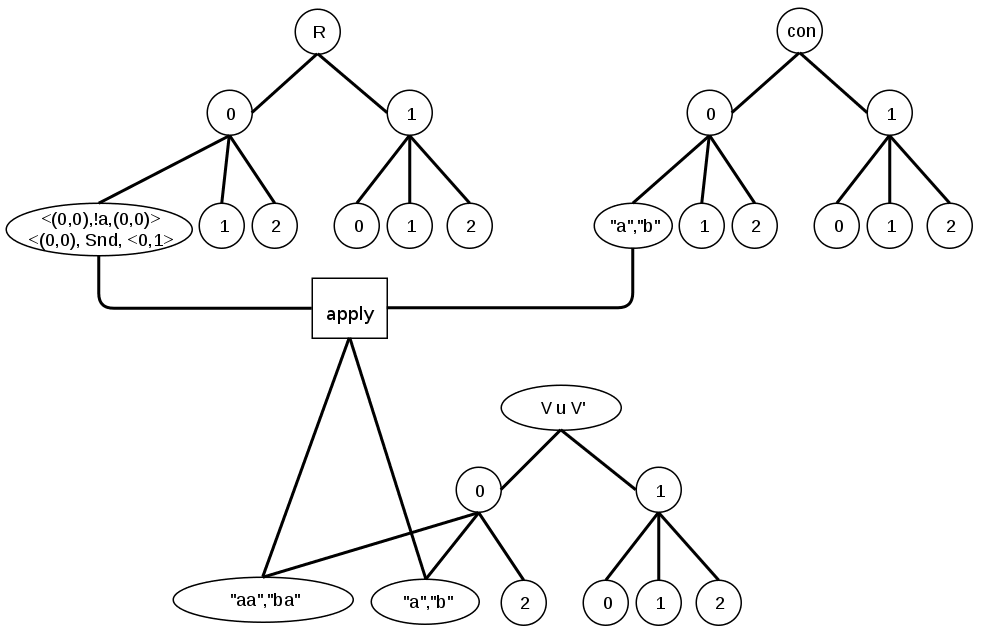
\includegraphics[width=400pt] {bilder/applyrule.png}
\caption{This picture shows the process of applying rules. For each control-state, each rules with that state are applied on each configuration with the same state. This will generate new configurations, not necessarily with the same control-state. For clarity.  tree structure is used to illustrate a hashmap.}
\label{applyrule}
\end{figure}



\subsection{Advantages of Partitioning}
Having partitioned the set $X$ of configurations into a hashmap of $X_k$ of sets, all set operations are made more effective. In a best-case scenario, there would be approximately the same number of configurations for every state in the system. The complexity of checking whether $\alpha_k(c)$ $\in$ $V$ is reduced to $O(log (n/|S|))$ where $S$ is the set of control-states in the system. The complexity of inserting an element is naturally the same.

Additionally, the complexity of calculating the set of post-images of a set $\gamma_k^{k+1}(X)$ is reduced, as we need not perform the calculation of each each $\rho = (s, op, s') \in \delta$ on each $c \in \gamma_k^{k+1}(X)$, but only on the subset of configurations for which $state(c) = s$.


\begin{algorithm}
  \caption{The verification algorithm from section \ref{alg1} in somewhat higher detail. This version includes }\label{euclid}
  \begin{algorithmic}[1]
    \State \textbf{Gamma (V, Seen):}
    \State \hspace{6 mm} con' := concretizations (V)
    \State \hspace{6 mm} con  := c | c $\in$ con $\land$ c $\notin$ Seen
    \\
    \State \textbf{Step (Con, Rules):}
    \For {state $\in$ nodes(V)}
    \State \hspace{6 mm} S := r(c) | $\forall$ c $\in$ con(state) $\land$ $\forall$ r $\in$ Rules(state)
    \EndFor
    \\
    \State \textbf{Alpha (V, S):}
    \State \hspace{6 mm} V:= V $\cup$ views(C)
    \\
    \State \textbf{Verifier (V, Rules, Bad):}
    \For{\texttt{$True$}}
        \If {$\mathcal{R}_k$ $\cap$ $Bad$ $\neq$ $\emptyset$}
        \State return Unsafe
        \EndIf
        \State V := $\mu Alpha(Step(Gamma(V)))$
        \If {$\gamma_k(V)$ $\cap$ $Bad$ = $\emptyset$}
        \State return Safe
        \EndIf
        \State k := k+1
      \EndFor
\end{algorithmic}
\end{algorithm}



\newpage
\section{Final Implementation}
An efficient algorithm in this context is largely an algorithm that avoids performing unnecessary calculations. This can either be done by avoiding to create unnecessary configurations such as was done with the rule hashmap above or by avoiding re-calculating previously calculated results. The algorithm as described above reproduces its steps each iteration; if a configuration \e{c} can be extended to a concretization \e{con} at any point in the verification process, then \e{con} can and will be created in every following iteration. This includes checking whether \e{$\alpha_k(con) \subset V$}, applying a set of rules to the configuration and then adding all the views of the resulting configurations to the set. Each time the calculations are performed, the result will be duplicates and no new views are added to the system.

We solve this by maintaining another hashmap, \e{seen}, of configurations in parallell, containing exactly those concretization that have been accepted. If a configuration \e{c} can be extended to the concretization \e{con}, then we first check if \e{con} is an element of seen. If it is, we discard \e{con}, otherwise we add \e{con} to \e{seen} and also to the set of concretizations to be evaluated in this iteration.

Yet another source of repetition is the fact that there are multiple ways to create the same channel evaluations. Therefore, after a rule has been applied to a concretization, it may result in a configuration already in the set. Instead of performing the costly $\alpha$-calculation, we first check if the newly created configuration is not in fact a duplicate by checking if it is already in \e{V}. If so, the configuration can again be discarded.

The final algorithm amounts to the following pseudo-code representation:

\subsection{Reachability Analysis}
An important step of the verification process which has yet to be covered is that of performing a reachability analaysis, in order to find bad states, if any such states are reachable and find a minimal bad trace leading up to the bad state. See sections \ref{bad} and \ref{traces} for formal definitions of bad states and traces respectively.

Below, a simple technique of finding a minimal bad trace is presented, accompanied with a proof that the trace is in fact minimal.

\subparagraph{Finding Minimal Traces}
When running the verification, if a bad state is found we want to produce a trace leading up to the bad state. Preferably, this would be a minimal trace that leads to the bad state.

The proposed verification method generates a finite set of reachable states (nodes in this context), but it does not record the available transitions between the nodes (i.e. the edges). It is possible to for each node \e{n} to save all nodes \e{n} from which an edge to \e{n'} exists, and thus build the complete reachability graph of the problem. There exists efficient algorithms to solve such a problem, e.g. \e{dijkstra shortest path}, or even the shortest path between any two nodes, e.g. flow-network techniques. Although these algorithms are efficient, building the complete reachability graph would be costly in terms of memory space, as the number of edges may be much larger than the number of states.


We show that due to the method of iteratively constructing the graph, nodes are created in such a way, that if a node $n_{i}$ created in the \e{i}:th iteration is reached by a node $n_{i-1}$ over an edge $e_{i-1}$, the shortest path from the initial node $n_0$ will necessarily be a path $e_1...e_{i-1}$.

\e{Proof.} This is proven using an induction proof. We hypothesize that, if at the point of creation of $n_i$, choosing the parent node $n_{i-1}$ from which an edge $e_{i-1}$ can be taken $n_i$, the path $e_1..e_{i}$ will be the shortest path to $n_i$ and has length \e{i}. Note that the node $n_{i-1}$ must have been created in the previous iteration; had it been created earlier, the edge $e_i$ could have been taken in a previous iteration, and so $n_{i+1}$ would already be a node in the tree.

The base case is that for any node reachable from $n_0$ over any edge $e_0$, $e_0$ will be the shortest path and has length 1. This is trivially true.

Now suppose a node $n_{i+1}$ is reachable over an edge $e_i$ from a node $n_i$, and the node $n_{i+1}$ is not yet in the system. The induction hypothesis states that the path $e_1...e_i$ is the shortest path leading up to $n_i$. If $e_0..e_{i-1}e_i$ would not be the shortest path to $n_{i+1}$, there would be a path $e'_0..e'_{k-1}$ to another node $n_k$ with k < i from which $n_{i+1}$ can be reached. But any such node would have been created in the \e{k}:th iteration of the algorithm, which would contradict the fact that the node $n_{i+1}$ was not already in the system.

Having shown this, we need only record the information of a single parent of a node, in order to build up a tree from which the shortest path from $n_0$ to any node in the system can efficiently be found.


\subsection{Specification Language}
\label{speclang}
In order for the verification algorithm to be easily used, a specification language is needed in which algorithms can be formally defined. We expect such a specification language to

\begin{itemize}
\item
be expressive enough to express all algorithms that are in the scope of the verification program
\item
be independent of the internal representations of the verifier and to demand as little knowledge of the actual verification process as possible from the user
\item
to be as clear as possible in order to ensure that the model at hand in fact corresponds to the actual algorithm, the way it was intended
\end{itemize}

The specification language used is an adaption of previous works in \cite{mpass}. The language simply uses XML to describe an algorithm. There are minor differences between the specification language used here, with respect to that used in by the MPass verification algorithm, and correspond to different expressivness of the models. More specifically, the MPass verifier allows for joint reception and transmission transitions, i.e. a single transition may read a message from a channel and write a message to a channel at the same time. On the other hand, it does not allow for synchronized transitions, this has therefore been added to the language.

\subsubsection{Example}
We return yet again to the Alternating Bit Protocol to examplify the specification language. Bearing in mind the formal definition in section \ref{CS}, a model needs a set of messages, channels, actions and transitions.

We begin by specifying a new protocol, it's name and that it is operating on FIFO buffers. We then specify a set of messages, a set of channels and a set of actions in a similar manner.

\lstset{language=XML}
\begin{lstlisting}[frame=single]
<protocol name="Alternating Bit Protocol" medium="FIFO>
<messages>
      <message>ack0</message>
      <message>ack1</message>
      <message>mesg0</message>
      <message>mesg1</message>
</messages>

<channels>
      <channel>c1</channel>
      <channel>c2</channel>
</channels>

<actions>
      <action>Rcv</action>
      <action>Snd</action>
</actions>
\end{lstlisting}

We then continue by defining the different processes in the system, i.e. the sender, receiver and observer. Such a process is defined by its states and its transitions. In the specification language, we differentiate between transitions over an action, and transitions that modify a channel. The latter type is called a \e{rule} in the specification language, in order to comply with the names used in the MPass specification language. This should not be confused with the word as used earlier in this section.

\begin{lstlisting}[frame=single]
  <role name="SENDER">
    <states>
      <state type="initial">Q0</state>
      <state>Q1</state>
      <state>Q2</state>
      <state>Q3</state>
    </states>
    <action>
        <current_state>Q0</current_state>
        <type>Snd</type>
        <next_state>Q1</next_state>
    </action>
    <rule>
        <current_state>Q1</current_state>
        <send_message>mesg0</send_message>
        <next_state>Q1</next_state>
        <channel>c1</channel>
    </rule>
\end{lstlisting}

Last, we specify that the processes \texttt{SENDER} and \texttt{OBSERVER}, and  \texttt{RECEIVER} and \texttt{OBSERVER} are to be synchronized over the actions \texttt{Snd} and \texttt{Rcv} respectively.

\begin{lstlisting}[frame=single]
<synchronize>
        <first_role>SENDER</first_role>
        <second_role>OBSERVER</second_role>
        <action>Snd</action>
</synchronize>
<synchronize>
        <first_role>RECEIVER</first_role>
        <second_role>OBSERVER</second_role>
        <action>Rcv</action>
</synchronize>
\end{lstlisting}
